\section{Progettazione}
Nella fase iniziale, il gruppo ha deciso come strutturare il sito, sia dal per l'amministratore, che per l'utente visitatore, in base degli obiettivi prefissati e alle linee guida da seguire.\\
È stata definito lo schema generale del database, pensandolo nella maniera più mantenibile per sviluppi futuri. \\
Successivamente sono stati definiti i diversi layout per ogni pagina del sito, pensando ai diversi schermi di visualizzazione.\\Pianificando gli obiettivi, sono stati suddivisi i compiti tra i membri del gruppo.

\subsection{Classificazione degli utenti}
I tipi di utente sono:
\begin{enumerate}
\item \textbf{cliente}, \\ovvero l'utente interessato ai contenuti del sito, quindi:
\begin{itemize}
\item può visualizzare i lavori che la fioreria produce, anche nel dettaglio;
\item tramite la pagina contatti, può: 
\begin{itemize}
\item visualizzare tutte le informazioni identificative riguardo la fioreria;
\item contattare l'amministratore tramite un apposito form;
\end{itemize}  
\end{itemize}  
\item \textbf{admin}, \\ovvero l'utente interessato alla gestione dei contenuti del sito, quindi:
\begin{itemize}
\item può gestire le richieste che i clienti mandano tramite l'apposito form; 
\item può gestire le categorie di lavori:
\begin{itemize}
\item creare una nuova categoria di lavoro;
\item modificare i dati di una nuova categoria di lavoro già inserita;
\item eliminare una categoria di lavoro già inserita;
\end{itemize} 
\item può gestire gli orari del pubblico da mostrare;
\item può gestire gli altri amministratori del sito, e eventualmente aggiungerne uno;
\end{itemize}
Credenziali degli utenti admin inseriti:
\begin{center}
\begin{tabular}{|p{0.2\textwidth}|p{0.2\textwidth}|}
\hline
username          & password        \\
\hline
admin           & admin     \\
admin2         & admin2     \\
admin3         & admin3     \\
prova         & prova     \\
\hline
\end{tabular}
\end{center}
\end{enumerate}

\subsection{Database}
Viene ora mostrata la struttura del database del sito, il quale permetterà la gestione degli utenti admin, delle richieste inviate dai clienti, delle impostazioni e dei vari lavori. Ogni lavoro ha più di un'immagine, mentre un'immagine può appartenere ad un solo lavoro.\\C'è poi una tabella per la gestione delle richieste dei clienti, una per la gestione degli admin e una per le impostazioni, ovvero le informazioni tecniche dell'azienda.
\begin{center}
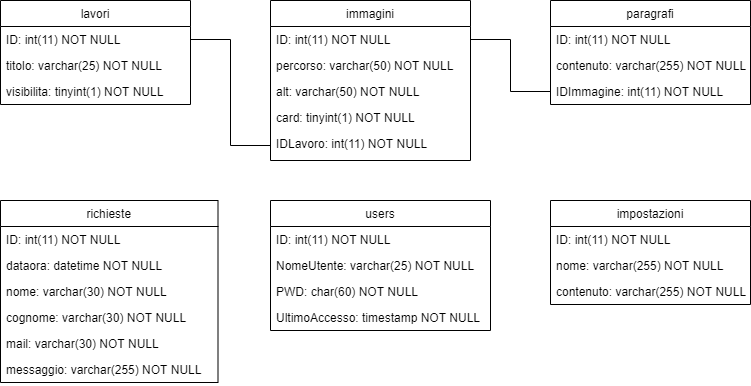
\includegraphics[scale = 0.5]{../latex/images/db.png}\\[1.5cm]
\end{center}

\subsection{Struttura dei contenuti}
dire che c'è lato clienti e lato admin.

\subsubsection{Lato cliente}
qualcosa qualcosa qualcosa qualcosa qualcosa qualcosa qualcosa qualcosa qualcosa qualcosa qualcosa qualcosa qualcosa qualcosa.\\\\
\textbf{Pagine}\\
qualcosa qualcosa qualcosa qualcosa	
	\begin{itemize}
		\item \textbf{Home} \\qualcosa qualcosa
		\item \textbf{Chi siamo}\\qualcosa qualcosa
		\item \textbf{Lavori}\\dire le pagine che lo compongono e cosa contengono
	 	\begin{itemize}
 			\item Matrimoni;\\	qualcosa qualcosa 
	 		\item Lauree;\\	qualcosa qualcosa 
 			\item Funerali;\\	qualcosa qualcosa
 			\item ...; 		 		
	 	\end{itemize}
	 	\item \textbf{Contatti}\\qualcosa qualcosa\\
 	\end{itemize}
\textbf{Parti fondamentali -> troviamoci un sinonimo}\\ 
	qualcosa qualcosa qualcosa
	\begin{itemize}
		\item \textbf{Header}\\qualcosa qualcosa
		\item \textbf{Breadcrumb}\\qualcosa qualcosa
		\item \textbf{Footer}\\qualcosa qualcosa
 	\end{itemize}
 		
\subsubsection{Lato Admin}
Come prima cosa è bene precisare che tutti gli admin inseriti hanno tutti gli stessi permessi sulla gestione di tutto il sistema. Questo è stato fatto perchè ad avere accesso all'interfaccia di amministrazione saranno un numero ristretto di fidate persone.\\
- discorso login\\
- discorso session\\\\
\textbf{Pagine}\\ qualcosa qualcosa qualcosa
	\begin{itemize}
		\item \textbf{Dashboard};\\qualcosa qualcosa
		\item \textbf{Gestione richieste};\\qualcosa qualcosa
		\item \textbf{Gestione categorie};\\dire le pagine che lo compongono e come funziona il tutto
	 	\begin{itemize}
 			\item Aggiungi categoria;\\qualcosa qualcosa
 			\item Modifica categoria;\\qualcosa qualcosa
 			\item Elimina categoria;\\qualcosa qualcosa
	 	\end{itemize}
 	\item \textbf{Gestione utenti}\\qualcosa qualcosa qualcosa
 	\item \textbf{Logout}\\qualcosa qualcosa qualcosa\\
 	\end{itemize}
\textbf{Parti fondamentali -> troviamoci un sinonimo} \\
\begin{itemize}
	\item \textbf{Breadcrumb}\\	qualcosa qualcosa qualcosa
	\item \textbf{Funzionamento PHP}\\	DbConnection ecc.
\end{itemize}